\chapter{Einführung}

\section{Organisatorisches}

\begin{itemize}
	\item Klausur: Schriftlich, 2 Stunden, davon $\frac{1}{3}$ Analysis, $\frac{2}{3}$ Algebra
	\item Hilfsmaterialen: Kein Taschenrechner, jeweils 1 handbeschriebenes A4-Blatt
	\item Online-Materialen: \href{https://drive.google.com/drive/folders/1CJ0226zg1_bnbt7IopCLwDuK2hkOgHya?usp=sharing}{drive.google.com}
	\item \LaTeX-Quellcode und weiteres: \href{https://github.com/blutorange/ba-dresden-calculus-awa}{github:blutorange/ba-dresden-calculus-awa}
	\item Kontakt: \href{mailto:wachsmuth.andre@gmx.de?subject=BA/Analysis 2020: }{wachsmuth.andre@gmx.de}
	\item Buchempfehlung: Meyers kleine Enzyklopädie der Mathematik, hrsg. von Siegried Gottwald, Meyers Lexikonverlag, \href{https://www.amazon.de/-/en/Siegfried-Gottwald/dp/3411077719}{ISBN-3 3-411-07771-9}
	\item Buchempfehlung: Repetitorium der höheren Mathematik, Merziger / Wirth, Binomi-Verlag, \href{https://www.amazon.de/-/en/Gerhard-Merziger/dp/3923923333}{ISBN-3 3-923-923-33-3}
\end{itemize}

\section{Anwendungen der Mathematik}

Mathematik stärkt die Fähigkeit zur Abstraktion und hilft bei der Lösung komplexer, auch nicht-mathematischer, Probleme. Grundlegend
ist die Fähigkeit, ein Problem analysieren zu können, es in Unterprobleme zu teilen und eine Lösungsstrategie zu erarbeiten zu können.

Auch in der Informatik und Programmierung sind mathematische Konzepte in einem breiten Umfang relevant.

\begin{itemize}
	\item In der objektorientierten Programmierung gibt es den Begriff der "Datenklassen". Um zu definieren, wie man diese vergleicht (\#equals) und ordnet (\#compareTo), werden Konzepte aus der Theorie der Relationen benötigt.
	\item Die Graphentheorie spielt eine wichtige Rollen bei Datenstrukturen und Algorithmen. Binäre Bäume stellen eine wichtige Datenstruktur für die effiziente Berechnung dar, gewichtete Graphen sind von wichtiger Bedeutung für das Problem des Handelsreisenden (Traveling Salesman), welches Anwendung findet in der Routenplanung, der Netzwerkarchitektur oder der Schaltkreisplanung.
	\item Grenzwertbetrachtungen und sogenannte Landau-Symbole werden genutzt, um die Laufzeit und den Speicherverbrauch von Algorithmen zu analysieren und zu beschreiben.
	\item Die Kategorientheorie ist eine Grundlage für algebraische Datenstrukturen. Zusammen mit dem $\lambda$-Kalkül stellen Sie die Basis funktionaler Programmierung dar.
	\item Die kontinuierliche Mathematik und die Infinitesimalrechnung stellen den Grundbaustein dar für physikalische Simulationen (Windtunnel, Crash-Test, Physics-Engine) und computergestützte Ingenieurswissenschaften (Gebäudestatik, Hydrodynamik, Schaltkreissimulation).
\end{itemize}

\section{Zahlenbereiche}

Grundlage für die gesamte Analysis die Objekte, auf denen sie operiert: Zahlen und Zahlenmengen. Zahlen modellieren quantitative Zusammenhänge der realen Welt. Gleichartige Zahlen abstrahiert man als eine Menge zu Zahlenbereichen.


\begin{definition}{Menge}{Set}
	Eine Menge ist eine Sammlung verschiedenartiger Elemente. Irrelevant hierbei ist die Reihenfolge der Elemente.
\end{definition}

Bei obiger Definition handelt es sich um den sogenannten naiven Mengenbegriff. Es hat sich gezeigt, dass diese naive Vorstellung zu Widersprüchen führen kann,
weshalb präzisere Formulierungen der Mengentheorie gefunden wurden (etwa Zermelo–Fraenkel-Mengenlehre). Für diese Vorlesung ist der naive Mengenbegriff allerdings
ausreichend.

Bei der Definition der Zahlenbereich beginnt man mit den natürlichen Zahlen und erweitert diese dann schrittweise.

\begin{definition}{Natürliche Zahlen}{NatNum}
	Die natürlichen Zahlen sind die Menge $\N$, die man erhält, wenn man mit dem Element $0$ beginnt und weitere Elemente rekursiv durch Bildung des Nachfolgers bestimmt.
\end{definition}

Präzisiert wird diese Definition durch die sogenannten \mention{Peano}-Axiome. Dabei kann man $0$ etwa mit dem Element $\setzero$ (leere Menge) identifzieren und die Nachfolgerbildung mit der Zuweisung
$\setzero \mapsto \lbrace \setzero \rbrace$ (Menge mit der leeren Menge). Der Vollständigkeit halber seien diese Axiome hier kurz angegeben.

\begin{definition}{\mention{Peano}-Axiome}{PeanoAx}
	\begin{enumerate}
		\item 0 ist eine Zahl.
		\item Jede Zahl $n$ hat genau einen Nachfolger $n'$.
		\item $0$ ist nicht Nachfolger einer Zahl.
		\item Jede Zahl ist Nachfolger höchstens einer Zahl.
		\item Von allen Mengen, die die Zahl $0$ und mit der Zahl $n$ auch deren Nachfolger $n'$ enthalten, ist die Menge $\N$ der natürlichen Zahlen diejenige mit den wenigsten Elementen.
	\end{enumerate}
\end{definition}

Natürliche Zahlen gibt es in zwei Ausprägungen. Die sogenannten \mention{Kardinalzahlen} beschreiben eine Anzahl, etwa die Anzahl von Büchern in einem Korb oder die Elemente in einem Array (Array-Länge).
Hinzu kommen die $\mention{Ordinalzahlen}$, welche eine Ordnung oder Rangfolge beschreiben. Im Gegensatz zu den Kardinalzahlen kann der Anfang bei Ordinalzahlen beliebig gewählt werden. Man kann den Index eines
Arrays sowohl bei $0$ als auch bei $1$ beginnen lassen, in beiden Fällen wird damit das \emph{erste} Element bezeichnet.

Nun reichen die natürlichen Zahlen nicht aus, um alle Gegebenheiten zu modellieren. Etwa ist es damit umständlich, Einnahmen und Kosten zu beschreiben. Hier müsste man immer angeben, ob es sich bei einer Quantität umd Einnahmen oder Kosten handelt und Regeln festlegen, wie Einnahmen und Kosten miteinander zu verrechnen sind. Um solche Gegensätze besser beschreiben zu können, führt man die ganzen Zahlen ein.
Kosten sind nun einfach beschreibbar als negative Einnahmen. Mathematisch motiviert werden die ganzen Zahlen, um ein inverses Element bezüglich der Addition angeben zu können. Dies wird unter dem Themengebiert siehe algebraische Strukturen im Modul Algebra näher beleuchtet.

\begin{definition}{Ganze Zahlen}{WholeNum}
	Die ganzen Zahlen sind die Menge $\Z$, die man aus $\N$ gewinnt, wenn man zu jeder natürlichen Zahl $n$ noch ihr Inverses $n'$ hinzunimmt. Dabei gilt $n+n' = n+(-n) = 0$.
\end{definition}

Doch auch die ganzen Zahlen sind unzureichend, um Verhältnisse und Verteilungen. Um etwa die Verteilung eines Geburtstagskuchen zu beschreiben, muss man immer die Grundgesamtheit (12 Stücke) als auch den Anteil
davon (3 Stück) angeben. Dies ist umständlich, stellt aber die Idee für die Definition der gebrochenen Zahlen dar.

\begin{definition}{Gebrochene Zahlen}{RatNum}
	Die gebrochenen Zahlen sind die Menge $\Q$, welche aus Paaren $(p,q) \in \Z^2$ ganzer Zahlen besteht. $p$ bezeichnet man dabei als Zähler, $q$ als Nenner. Zwei ganze Zahlen heißen äquivalent,  wenn
	diese den gleichen Bruch darstellen, also wenn gilt: $(p,q) \equiv (p',q') \iff pq'=p'q$	
\end{definition}

Solche Brüche werden in der Informatik verwendet, um Fehler bei der Addition und Multiplikation zu vermeiden. Dies ist für einige Anwendungsbereiche wie Finanzen von wichtiger Bedeutung, um Geldbeträge
Cent-genau berechnen zu können. Ein Spezialfall davon ist die sogenannte Festkommazahlrechnung (fixed-point arithmetics), wobei der Nenner immer fest vorgeben ist.

Nun gibt es auch Rechenaufgaben, die selbst durch gebrochene Zahlen nicht gelöst werden können. Beispielsweise hat $x^2=2$ keine Lösung im Bereich der gebrochenen Zahlen. Allerdings ist es möglich,
Näherungswerte als Brüche anzugeben: $\frac{3}{2}, \frac{17}{12},\frac{577}{408}$. Man sieht hier, dass die Näherungswerte besser werden, also näher an der gesuchten Lösung liegen. Tatsächlich kann man
eine Formel angeben, um immer bessere Näherungswerte für $x^2=2$ zu finden. Alle diese Näherungswerte sind gebrochene Zahlen, dennoch gibt es keine gebrochene Zahl mit der Eigenschaft $x^2=2$.

\begin{definition}{Fundamentalfolge}{CauchySeq}
	Eine Fundamentalfolge (Cauchy-Folge) ist eine Zahlenfolge $a_i$, bei der der Abstand der zweier Folgenglieder beliebig klein wird: $\forall \epsilon > 0: \exists N \in \N: \forall m,q>N: |a_m-a_q|<\epsilon$
\end{definition}

Wie eben anhand des Beispiels $x^2=2$ illustriert, gibt es im Bereich der rationalen Zahlen Fundamentalfolgen, die sich zwar scheinbar einem Wert zu nähern scheinen (die also eine Cauchy-Folge darstellen),
wobei dieser Wert selber allerdings keine gebrochene Zahl ist. Zur Lösung dieses Problems werden die reellen Zahlen definiert.

\begin{definition}{Reelle Zahlen}{RealNum}
	Die reellen Zahlen sind die Menge $\R$, welche aus allen Fundamentalfolgen $a_i$ ganzer Zahlen besteht. Zwei Fundamentalfolgen $a_i, b_i$ sind dabei äquivalent, wenn $|a_i-b_i$ eine Nullfolge bildet.
\end{definition}

Tatsächlich lässt sich zeigen, dass auf der Menge der reellen Zahlen $\R$ jede Cauchy-Folge konvergiert, also einen Grenzwert besitzt. Die reellen Zahlen sind im Gegensatz zu den gebrochenen Zahlen \emph{vollständig}.

Als Erweiterung der reellen Zahlen gibt es noch die komplexen Zahlen $\C$, wobei ein neues Element $j$ mit der Eigenschaft $j^2=-1$ eingeführt wird, welches die sogenannte imaginäre Einheit heißt. Komplexe
Zahlen eignen sich beispielsweise, um Schwingungen zu beschreiben oder Strom- und Spannungsberechnungen an Schaltkreisen anzustellen. Solche komplexen Zahlen werden in der Algebra genauer betrachtet. Diese Vorlesung beschränkt sich auf die reellwertige Analysis. 

\section{Operationen und Rechenregeln}

Auf den Zahlenbereichen werden Rechenoperationen definiert, welche gewisse Regeln genügen. Die systematische Beschreibung solcher Rechenoperationen erfolgt durch das Gebiet algebraische Strukturen im Modul Algebra. Für die Analysis wird vorausgesetzt, dass elementare Rechenregeln aus Sekundarstufe I und II sowie der Umgang und die Umformung mathematischer Terme beherrscht werden. Im folgenden findet sich eine unvollständige Auflistung einiger wesentlicher Regeln: 

\begin{statement}{Kommunikativgesetz}{CommLaw}
	Für $a,b\in\R$ gilt: $a + b = b + a$
\end{statement}

\begin{statement}{Assoziativgesetz}{AssLaw}
	Für $a,b\in\R$ gilt: $a + ( b + c) = (a + b) + c$
\end{statement}

\begin{statement}{Distributivgesetz}{DisLaw}
	Für $a,b,c\in\R$ gilt: $a \cdot ( b + c ) = a \cdot b + a \cdot c$
\end{statement}

\begin{statement}{Potenzgesetze}{PowerIds}
	Für $x, y, p,q\in\R$, für welche die Potenzen erklärt sind, gelten die folgenden Rechenregeln:
	\begin{itemize}
		\item $x^{p+q} = x^p \cdot x^q$
		\item $x^p \cdot y^p = (x \cdot y)^p$
		\item $x^{(y^z)} = x^{y \cdot z}$
	\end{itemize}
\end{statement}

\begin{statement}{Logarithmengesetze}{LogIds}
	Für $x, y\in\R$, für welche die Logarithmen erklärt sind, gelten die folgenden Rechenregeln:
	\begin{itemize}
		\item $\ln(x \cdot y) = \ln(x) + \ln(y)$
		\item $\ln(x^y) = y \ln(x)$
		\item $\log_y(x) = \ln(x) / \ln(y)$
	\end{itemize}
\end{statement}

Für die Operationen $+$ (Addition) und $*$ (Multiplikation) gibt es zudem eine Kurzschreibweise, wenn eine (möglicherweise variable) Anzahl von Summanden addiert oder Faktoren multipliziert werden sollen. Man gibt dabei einen Laufindex an, der innerhalb gewisser Grenzen verläuft, und einen Term, in den jeder erlaubte Wert des Laufindex eingesetzt wird. Die Werte des Terms für jeden Laufindex werden dann addiert beziehungsweise multipliziert. Geschrieben wird dies wie folgt:

$$
\sum\limits_{i=1}^{10} i^2  \\
$$

$$
\prod\limits_{i=1}^{5} i 
$$

Oben steht eine Summe ($\Sigma$ für Sigma, Summe), gesprochen: "Die Summe von i gleich 1 bis 10 über i-Quadrat." Es sollen also die ersten 10 Quadratzahlen addiert werden. Unten steht ein Produkt ($\Pi$ für Pi, Produkt), gesprochen: "Das Produkt von i gleich 1 bis 5 über i." Hier sollen also die Zahlen von $1$ bis $5$ multipliziert werden ($=5!$). Man beachte auch die Analogie zu einer \emph{For-Schleife} in der Programmierung:

\begin{jscode}
sum = 0;
for (i = 1; i <= 10; ++i)
	sum += i * i;
\end{jscode}

\section{Schlussfolgern}

Ein in der Schulmathematik häufig vernachlässigter wichtiger Bestandteil der Mathematik ist das Schlussfolgern, also dem Ziehen von Schlüssen basierend auf gewissen Grundannahmen oder Axiomen. Hierfür
gibt es einige wichtige Techniken wie \emph{Induktion} oder \emph{reductio ad absurdum}. Auch wenn das Beweisführen in dieser Vorlesung nicht im Vordergrund steht, wird erwartet, dass zu einer Antwort
immer eine knappe, aber fundierte Begründung (Rechenweg oder Prosa) gegeben wird. In folgenden wird anhand einiger Beispiele kurz illustriert, wie mathematische Beweise geführt werden können.

\subsection{Beweis durch Widerspruch}

Frage: Ist $\sqrt{2}\in\Q$?

Wir nehmen an, $\sqrt{2}$ wäre eine gebrochene Zahl, also darstellbar als vollständig gekürzter Bruch $\frac{p}{q}, p,q\in\Z, p,q>0$. Dann sind $p$ und $q$ teilerfremd. Es folgt nun:

\begin{align}
  \sqrt{2} & = p / q \\
         2 & = p^2 / q^2 \\
     2 q^2 & = p^2 \label{eq:sqrt2-p2even}
\end{align}

Aus Gleichung \ref{eq:sqrt2-p2even} folgt, $p^2$ ist eine gerade Zahl, da es sich als das doppelte einer anderen ganzen Zahl $q^2$ darstellen lässt. Weiterhin ist damit auch $p$ eine gerade Zahl, da das Produkt zweiter ungerade Zahlen
immer ebenfalls eine ungerade Zahl ergibt. Wir können $p$ nun schreiben als $p = 2 n, n\in \Z$. Es ergibt sich:

\begin{align}
	2q^2 & = p^2 = p * p = (2n) \cdot (2n) \\
	q^2 & = 2 n^2 \label{eq:sqrt2-q2even}
\end{align}
	
Da $n$ eine ganze Zahl ist, so ist auch $n^2$ eine ganze Zahl. Wegen \ref{eq:sqrt2-q2even} lässt sich $q^2$ sich schreiben als das doppelte einer ganzen Zahl und ist daher eine gerade Zahl, mithin ist also auch $q$ eine gerade Zahl.

Nun haben wir damit aber gezeigt, dass sowohl $p$ als auch $q$ gerade Zahlen sind. Sie besitzen also beide den Teiler $2$. Dies widerspricht der Annahme, dass es einen vollständig gekürzten Bruch $p / q = \sqrt{2}$ gibt. Die Annahme, dass es einen solchen Bruch gibt, wurde damit zu einem Widerspruch (ad absurdum) geführt (reductio). Somit gibt es keine gebrochene Zahl $x$ mit der Eigenschaft $x^2=2$.

\subsection{Nichtkonstruktiver Beweis}

Frage: Gibt es zwei irrationale Zahlen $x,y\notin \Q$ so, dass deren Potenz $x^y\in \Q$ eine rationale Zahl ergibt?

Wir wählen $x=y=\sqrt{2}$. Nach dem Satz vom ausgeschlossenen Dritten ist eine Aussage entweder wahr oder falsch, das heißt entweder gilt $\sqrt{2}^{\sqrt{2}} \in \Q$ oder $\sqrt{2}^{\sqrt{2}}\notin\Q$. Wir betrachten beide Fälle:

\begin{itemize}
	\item $\sqrt{2}^{\sqrt{2}}\in\Q$: $\sqrt{2}$ ist wie eben gezeigt irrational, damit ist ein Beispiel für zwei solche Zahlen gefunden.

	\item $\sqrt{2}^{\sqrt{2}}\notin\Q$: Wir setzen $x' = \sqrt{2}^{\sqrt{2}}$ und $y'=\sqrt{2}$. Die Zahl $x'$ ist nach Annahme irrational und die Potenz $(\sqrt{2}^{\sqrt{2})^{\sqrt{2}}} = \sqrt{2}^{\sqrt{2}\sqrt{2}} = \sqrt{2}^2 = 2$ ist eine rationale Zahl.
\end{itemize}

Wir haben damit gezeigt, dass es wenigstens eine Paar zwei solcher Zahlen gibt, nämlich entweder $(x,y) = (\sqrt{2}, \sqrt{2})$ oder $(x,y) = (\sqrt{2}^{\sqrt{2}}, \sqrt{2})$. Dieser Beweis heißt deshalb nichtkonstruktiv, da er keine Möglichkeit bietet, zu bestimmen, welche Zahlen es tatsächlich sind.

\section{Struktur von Termen}

Um mathematische Ideen zu kommunizieren, ist eine Notation notwendig, die gewissen Regeln folgt. Um etwa die Idee zu beschreiben, dass die Summe zweier Zahlen in einer Menge enthalten sei, wird in der üblichen mathematischen Notation die Schreibweise $a+b\in\N$ verwendet. Wir an diesem Beispiel zu sehen, besteht die mathematische Notation also zum Einen aus Symbolen für mathematische Objekte und Operationen und zum Zweiten aus Regeln, wie diese Symbole angeordnet werden dürfen. Genau dies ist aber die Definition einer sogenannten \emph{formalen Sprache} mit Wörtern und einer Grammatik für die Bildung von Sätzen.

Man beachte die Analogie zu Programmiersprachen, auch diese stellen eine solche formale Sprache dar. Genauso wie ein Programm dargestellt werden kann als \emph{Syntaxbaum} ist dies auch mit einem mathematischen Ausdruck möglich. Ein Syntaxbaum beginnt immer an der Spitze mit der hauptsächlichen Operation, und verzweigt dann in die einzelnen Unteroperation. Wir betrachten als Beispiel zuerst das folgende Computerprogramm zur Berechnung der $n$.-ten Fibonacci-Zahl in Listing \ref{lst:JsFibonacci}.

\begin{listing}[H]
\caption{JavaScript-Programm zur Berechnung der n.-ten Fibonacci-Zahl}
\label{lst:JsFibonacci}
\begin{jscode}
function fibonacci(n) {
	let n_0 = 0;
	let n_1 = 1;
	while (n-- > 0) {
		const sum = n_0 + n_1;
		n_0 = n_1;
		n_1 = sum;
	}
	return n_0;
}
\end{jscode}
\end{listing}	


In oberster Ebene ist die Struktur dieses Programms eine \emph{Function Declaration}, bestehend aus einem Funktionsnamen, einem Argument und einem Funktionskörper. Der Funktionskörper selbst ist zuallererst ein \emph{Block Statement}, bestehend aus einer \emph{Statement List}. Das Statement auf Zeile 5, \lstinline{const sum = n_0 + n_1}, wiederum ist ein \emph{Variable Declaration}-Statement, bestehend aus einem \emph{Identifier} für den Variablennamen und einem \emph{Initializer} für den Wert der Variablen. Der \emph{Initializer} ist eine \emph{Sum Expression} (Summen-Ausdruck), der wiederum aus 2 Summanden besteht. Jeder Summand ist in diesem Fall ein \emph{Identifier} für den jeweiligen Variablennamen. Verbal formuliert mag diese Struktur nur schwer vorstellbar sein. Graphisch ist der Syntaxbaum auszugsweise in Abbildung \ref{fig:JsFibinacciBaumPart} dargestellt. Der vollständige Syntaxbaum findet sich in Abbildung \ref{fig:JsFibinacciBaum}.


\begin{figure}[h]
	\caption{Syntaxbaum zum JavaScript-Programm für Fibonacci-Zahlen (Auszug)}
	\label{fig:JsFibinacciBaumPart}
	\centering
	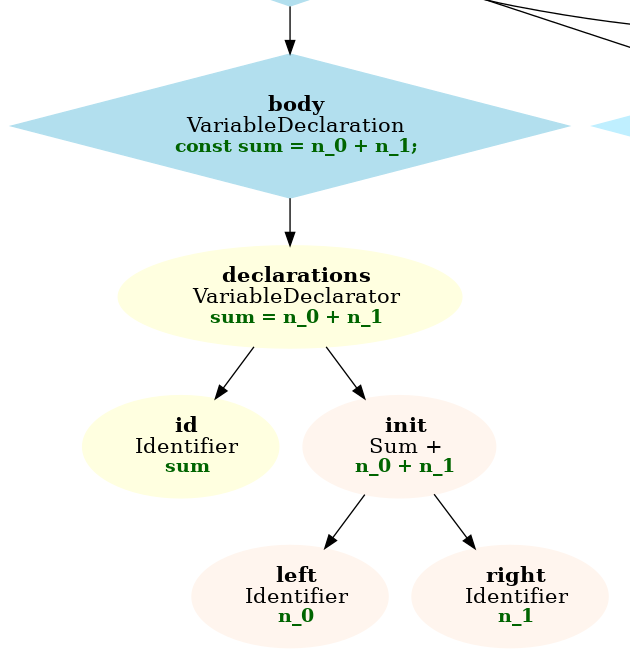
\includegraphics[width=0.5\textwidth]{./img/js-tree-fibonacci-part.png}
\end{figure}


\begin{figure}[p]
	\caption{Syntaxbaum zum JavaScript-Programm für Fibonacci-Zahlen}
	\label{fig:JsFibinacciBaum}
	\centering
	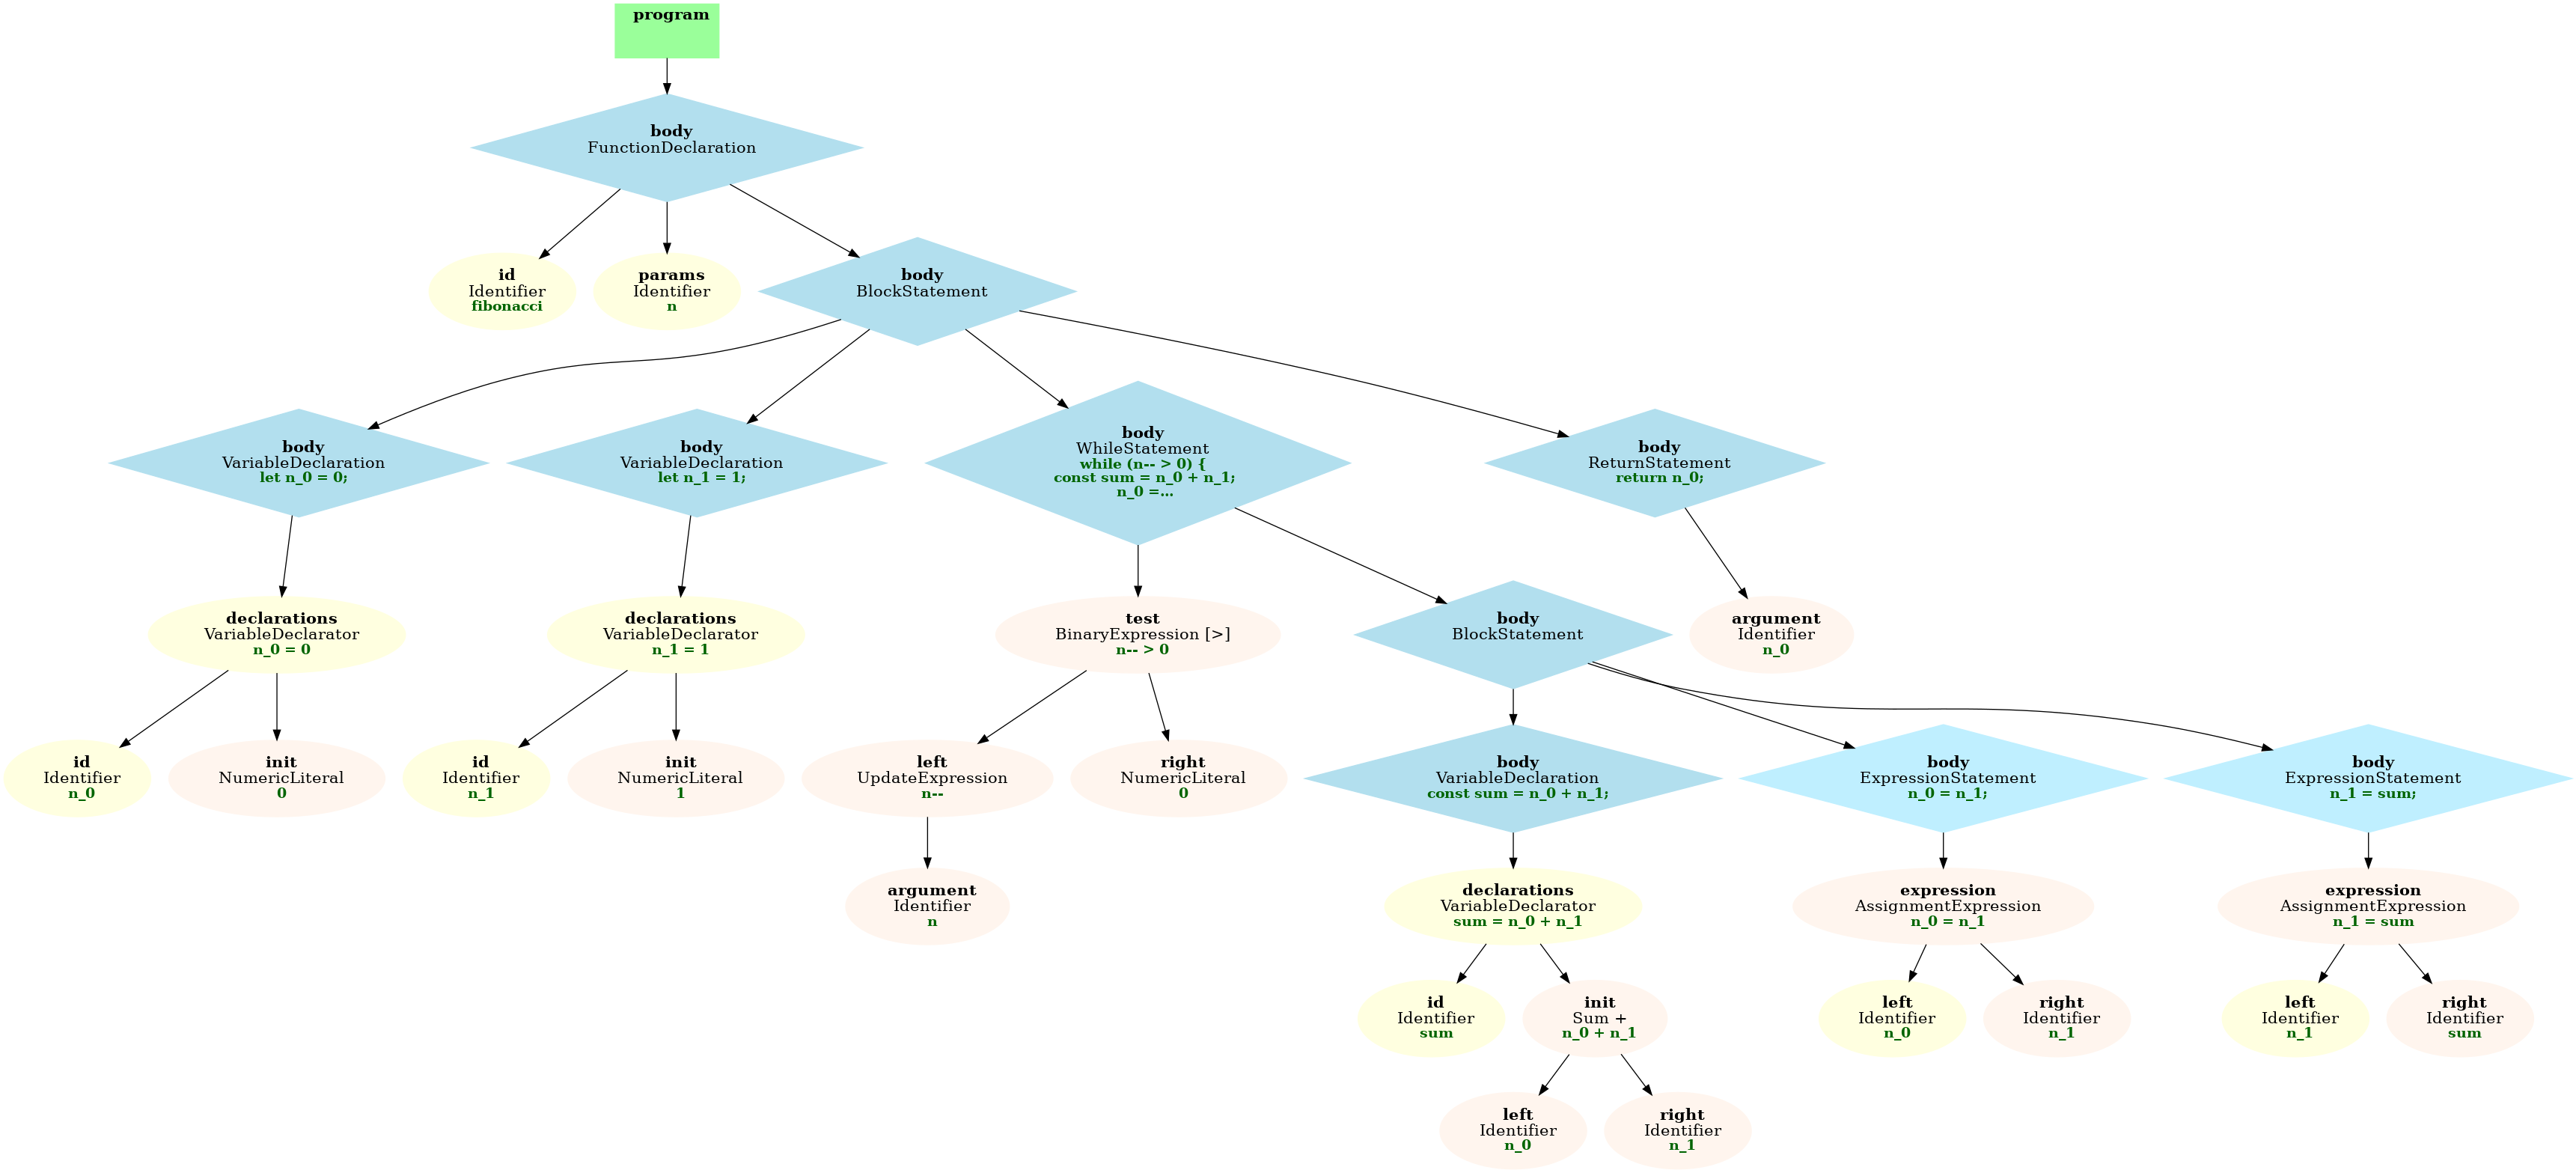
\includegraphics[width=0.95\textwidth]{./img/js-tree-fibonacci.png}
\end{figure}

Für die mathematische Notation besonders relevant sind die Ausdrücke (\emph{Expression}), also Rechenoperationen. Einen mathematischer Term lässt wie erwähnt als Syntaxbaum darstellen. Solch ein Syntaxbaum lässt sich schriftlich auf verschiedene Weisen schreiben. Die mathematische Notation lehnt sich an der sogenannten Infix-Notation an, wobei die Operatoren zwischen die Operanden geschrieben werden. Eine weitere Notation stellt die Polnische Notation dar, die etwa in manchen Taschenrechner verwendet wird und auch die Grundlage für \mention{Ldap}-Filter darstellt (Lightweight Directory Access Protocol). Wir wollen dies kurz am Beispiel $(a+b)\cdot(c+d)$ illustrieren. Der Syntaxbaum dazu ist zu finden in Abbildung \ref{fig:JsAbcdBaum}.

\begin{figure}[H]
	\caption{Syntaxbaum für $(a+b)(c+d)$}
	\label{fig:JsAbcdBaum}
	\centering
	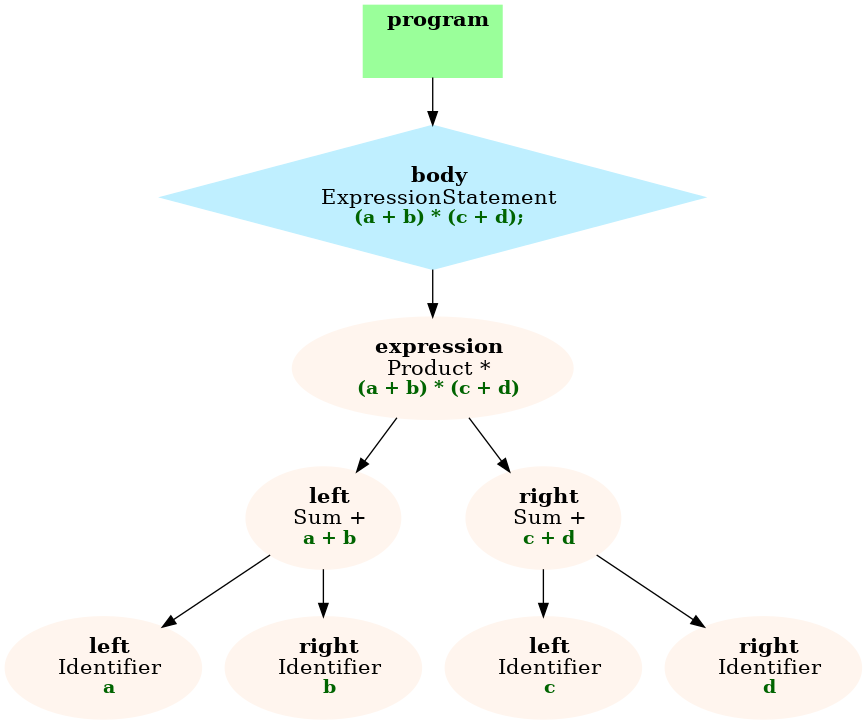
\includegraphics[width=0.5\textwidth]{./img/js-tree-abcd.png}
\end{figure}

Aus dem Syntaxbaum lesen wir ab, dass der Term aus der Hauptoperation \emph{Multiplikation} besteht. Die beiden Faktoren bestehen jeweils aus einer Unteroperation, hier einen Summenbildung. Die Infix-Notation $(a+b)\cdot(c+d)$ beginnt daher mit einem Multiplikationszeichen, zu dessen beiden Seiten Summenzeichen stehen. Um die Rangfolge zu wahren, welche durch den Syntaxbaum vorgegeben ist, erfordert die Infix-Notation die Verwendung von Klammerzeichen. Eine Alternative zur Infix-Notation ist die polnische Notation, welche keine Klammerzeichen benutzt und so etwa einfacher von Computerprogramme verstanden werden kann. Dies erreicht sie dadurch, indem sie zuerst für jeden Operator definiert, welche Arität (Anzahl von Operanden) er hat. Anschließend wird der Operator nicht zwischen die Operanden, sondern vor die Operanden geschrieben. Zusätzlich gibt es noch die sogenannte umgekehrte polnische Notation, wobei der Operator nicht vor, sondern nach den Operanden notiert wird. Für unser Beispiel $(a+b)(c+d)$ ist die polnische Notation dargestellt in Listing \ref{lst:PolAbcd}.

\begin{listing}[H]
	\caption{Polnische Notation (oben) und umgekehrte polnische Notation (unten)}
	\label{lst:PolAbcd}
\begin{textcode}
* + a b + c d
a b + c d + *
\end{textcode}
\end{listing}

Schließlich sei noch angemerkt, dass Rechenregeln sich darstellen lassen als Transformationen auf einem Syntaxbaum. Dies stellt die Grundlage dar für Computer-Algebra-System, welche auf symbolischen Ausdrücken arbeiten und diese umformen können. Dies ist in Abbildung \ref{fig:TreeTransformKommutativ} am Beispiel des Kommutativgesetzes dargestellt. Dieses besagt, dass bei einer \emph{Sum Expression} die beiden Unterbäume der beiden Summanden vertauscht werden können. Man beachte, dass die Summanden im Allgemeinen nicht Zahlen oder Variablen, sondern wiederum komplexe Baumstrukturen sind.

\begin{figure}[H]
	\caption{Syntaxbaumtransformation für das Kommutativgesetz}
	\label{fig:TreeTransformKommutativ}
	\centering
	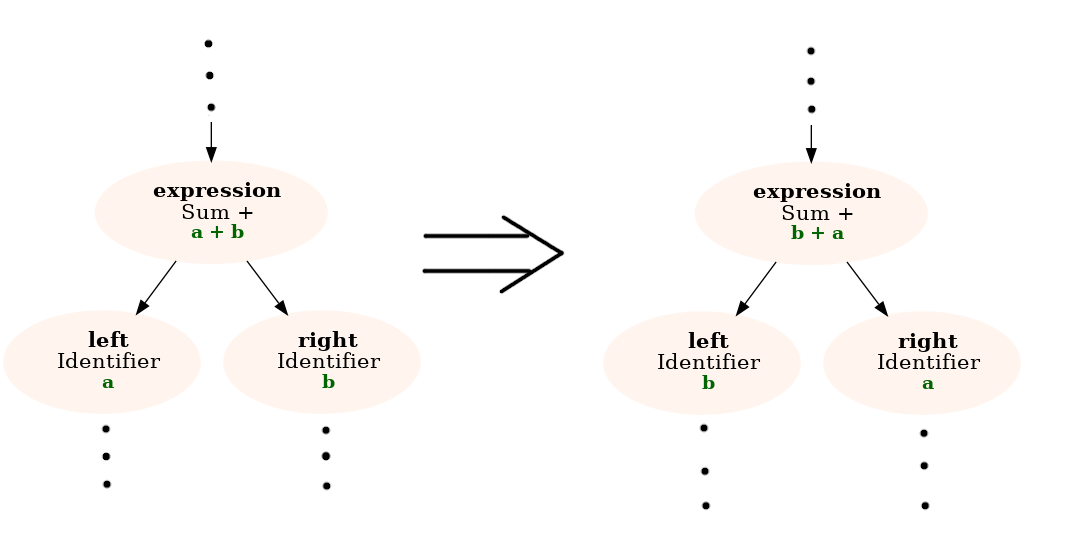
\includegraphics[width=0.8\textwidth]{./img/tree-transform.png}
\end{figure}